\documentclass[a4paper,utf8]{article}
\usepackage{graphicx}
\usepackage[heading,fancyhdr]{ctex}
\usepackage{amsmath,amssymb,geometry,ulem}
\usepackage{array,tabularx,tabulary,mhchem,xspace}
\usepackage{floatrow,subfig,multirow,bigstrut}
\usepackage{siunitx,booktabs,longtable,nameref}
\lineskiplimit=1pt
\lineskip=3pt
\geometry{
    top=25.4mm, 
    left=25mm, 
    right=25mm, 
    bottom=25mm,
    headsep=5.9mm,
}
\ctexset{
    chapter = {
        name = {实验,},
        beforeskip = {-23pt}
    }
}
\newcommand{\fgref}[1]{图~\ref{#1}\xspace}
\newcommand{\seqref}[1]{式~(\ref{#1})}
\newcommand{\expinfo}[6][无]{
    {\zihao{-3}\bfseries\songti
    实验名称:\uline{\hfill\mbox{#2}\hfill} \\[2.9mm]
    学\quad 号:\uline{\makebox[25mm]{#3}}\hfill
    姓\quad 名:\uline{\makebox[25mm]{#4}}\hfill
    班\quad 级:\uline{\makebox[25mm]{#5}} \\[2.9mm]
    合作者:\uline{\makebox[25mm]{#1}} \hfill
    桌\quad 号:\uline{\makebox[25mm]{}}\hfill\makebox[25mm+4em]{}\\[2.9mm]
    指导教师:\uline{\makebox[30mm]{#6}}\hfill\mbox{} \\[2.9mm]
    实验日期:\uline{\makebox[30mm]{}}\hfill\mbox{} \\[58.7mm]
    }
}%\expinfo[合作者]{实验名称}{学号}{姓名}{班级}{指导教师}
\newcommand{\pointingbox}{
    {\zihao{4}\bfseries\songti%
    实验考核\\[3mm]
    \extrarowheight=3mm
    \begin{tabularx}{150mm}{|X|X|X|X|X|}\hline
        \hfil 项目 \hfil  & \hfil 实验预习 \hfil & \hfil 实验过程 \hfil & \hfil 分析与讨论 \hfil & \hfil 总评 \hfil \\[3mm] \hline
        \hfil 评价 \hfil &  &  &  &  \\[3mm] \hline
    \end{tabularx}
    }
}
\newcommand{\derivative}[2]{\frac{\mathrm{d} #1}{\mathrm{d} #2}}
\newcommand{\thinking}[2]{\textbf{#1}\\
答:\begin{minipage}[t]{0.85\textwidth}
    #2
\end{minipage}}

\pagestyle{fancy}
\fancyhf{}
%\fancyhead[C]{材料科学基础实验}
%\fancyfoot[C]{\thepage}
\fancyhead[EC]{\leftmark} \fancyhead[OC]{\rightmark}
\fancyhead[EL,OR]{\thepage}
\fancypagestyle{plain}{\renewcommand{\headrulewidth}{0pt}\fancyhf{}}

\newcounter{Rownumber}
\newcommand*{\Rown}{\stepcounter{Rownumber}\theRownumber}
\newcounter{sample}
\newcommand*{\Sam}{\stepcounter{sample}\thesample}
\newcounter{Fignumber}
\newcommand*{\Fign}{\stepcounter{Fignumber}\theFignumber}

\newcommand*{\resetRown}{\setcounter{Rownumber}{0}}
\newcommand{\qrange}[3]{\qtyrange[range-phrase = \text{$\sim$},range-units =single]{#1}{#2}{#3}}
\floatsetup[table]{capposition=top}
\newcolumntype{C}{>{\hfil}X<{\hfil}}
\renewcommand{\Nameref}[1]{\textbf{\ref{#1}~\nameref{#1}}}
\newcommand{\TTR}[0]{\watt\per\m\per\K} %导入导言
\begin{document}
\begin{center}
    {\mbox{}\\[7em]\zihao{2}\bfseries\songti%
    材料科学基础实验报告}\\[34mm]
    \expinfo{铁碳合金的显微组织观察及性能分析}{22301077}{张蕴东}{22高分子}{杨玉华}
\end{center}
\newpage
\section{实验目的}
\begin{enumerate}
    \item 了解金相显微镜的成像基本原理、构造、主要部件及作用;
    \item 熟悉金相显微镜的使用和其注意事项;
    \item 掌握分析铁碳合金在平衡状态下及不同工艺热处理后的显微组织形态;
    \item 加深理解铁碳合金组织与性能之间的关系。
\end{enumerate}

\section{实验原理}%简单描述,含必要的公式和附图;
    \subsection{金相显微镜的成像原理}
        显微镜不似放大镜那样由单个透镜组成,而是由两级特定透镜所组成。靠近被观察物体的透镜叫做物镜,而靠近眼睛的透镜叫做目镜。借助物镜与目镜的两次放大,就能将物体放大到较高的倍数($\sim 2000$倍)。\fgref{fig:microscope} 所示是在显微镜中得到放大物像的光学原理图。被观察的物体 $AB$ 放在物镜之前距其焦距略远一些的位置,由物体反射的光线穿过物镜,经折射后得到一个放大的倒立实像 $A^{'}B^{'}$,目镜再将实像 $A^{'}B^{'}$ 放大成倒立虚像 $A^{''}B^{''}$,这就是我们在显微镜下研究实物时所观察到的经过二次放大后的物像。在设计显微镜时,让物镜放大后形成的实像 $A^{'}B^{'}$ 位于目镜的焦距 $f$ 目之内,并使最终的倒立虚像 $A^{''}B^{''}$ 在距眼睛 \SI{250}{\mm} 处成像,这时观察者看得最清晰。此时 $A^{''}B^{''}$ 的放大倍数是物镜放大倍数与目镜放大倍数的乘积。
        \begin{figure}[!ht]
            \caption{显微镜光学原理图\label{fig:microscope}}
            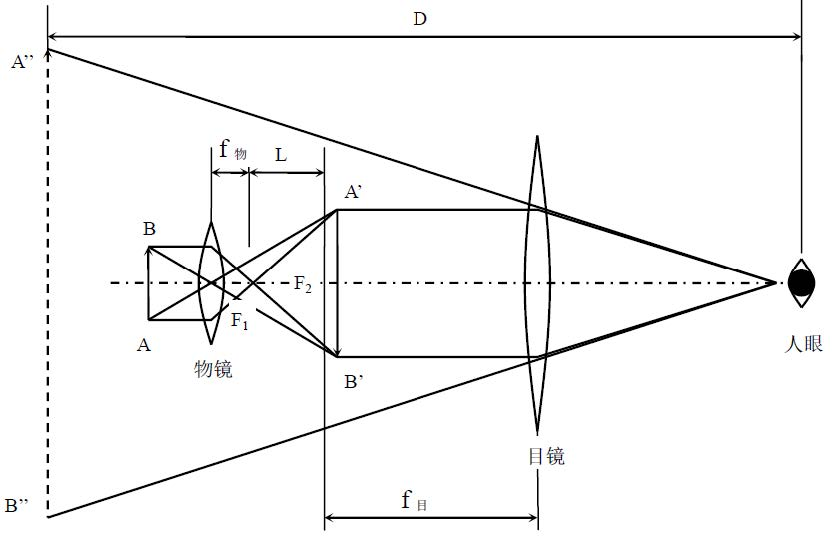
\includegraphics[width=0.7\textwidth]{microscope.jpg}
        \end{figure}\par
        显微镜的放大倍数为
        \begin{equation}
            M=M_\text{物}\cdot M_\text{目}\approx\frac{\Delta}{f_1}\cdot\frac D{f_2}
            \label{equ:1}
        \end{equation}\par
        式中:
        \begin{minipage}[t]{100mm}
            $M_\text{物}$-物镜的放大倍数;\par
            $M_\text{目}$-目镜的放大倍数;\par
            $f_1$-物镜的焦距;\par
            $f_2$-目镜的焦距;\par
            $\Delta$-显微镜的光学镜筒长(即物镜后焦点到所成实像的距离);\par
            $D$-人眼明视距离,约为 \SI{250}{\mm}。\par
        \end{minipage}
    \subsection{金相显微镜的构造}
        金相显微镜由照明系统、光学系统和机械系统三部分组成。另有一些显微镜还配有照相装置等附件。
        \subsubsection{照明系统}
            在显微镜底座内装有一个低压灯泡作为光源,与聚光镜、孔径光阑、视场光阑及反光镜组成显微镜的照明系统,使样品表面获得充分均匀的照明。
        \subsubsection{显微镜调焦装置}
            显微镜体两侧有粗调及微动调焦旋钮。转动粗调焦旋钮可使载物台迅速升降,微动调焦旋钮可使物镜缓慢地上下运动,以便精确调焦。
        \subsubsection{孔径光阑(AS)}
            光路中装有两个光阑。孔径光阑的作用是控制入射光束的大小,缩小孔径光阑可以减小像差,增大景深和衬度,使映像清晰。但随着孔径角的缩小,物镜的数值孔径降低,进而会使物镜的分辨能力降低;增大孔径光阑,入射光束变粗,物镜的孔径角增大,可使光线充满物镜的后透镜,数值孔径可达到物镜体上标刻的 NA 值,分辨率会随之提高。但由于球面像差的增加以及镜筒内部反射及炫光的增加,成像质量将降低。因此孔径光阑使用时需做适当的调节,实际操作中以在目镜筒内看到孔径光阑在物镜后焦面上成像达物镜孔径的 $80-90\%$ 时为好。更换物镜后,孔径光阑需做适当调节。另外,不应用它来调节视场的亮度。
        \subsubsection{视场光阑(FS)}
            通过调整视场光阑,可改变显微镜视场大小,可提高映像衬度而不影响物镜的分辨能力。适当调节视场光阑的大小还可减少镜筒内的反射及炫光,提高成像质量。但需注意视场光阑缩得太小,会使观察范围太窄,一般应调节到与目镜视场大小相同。
        \subsubsection{滤色片}
            滤色片是显微镜的辅助部件,通过合理选用可适当提高成像质量。滤色片是由不同颜色的光学玻璃片制成的透明薄片,目的是只允许一定波长的光线通过。其主要有以下几个作用:配合消色差物镜使用黄绿色滤色片,可使像差得到最大限度的校正;对复消色差物镜,可采用蓝色滤色片,由于蓝光波长较黄绿光短,因而可提高物镜的分辨率;减弱光源的强度等。
        \subsubsection{载物台}
            用于放置金相样品,观察面向下。通过调整纵向和横向移动手柄可使载物台在水平面上做一定范围的十字定向运动,以改变试样的观察部位。
        \subsubsection{物镜转换器}
            转换器可安装不同放大倍数的物镜,旋动转换器可使各物镜镜头进入光路,与不同的目镜搭配使用,以获得各种放大倍数。
        \par
        MDS400 倒置式金相显微镜的外形构造请见\fgref{fig:MDS400}。
        \begin{figure}[!ht]
            \caption{MDS400 倒置式金相显微镜的外形构造\label{fig:MDS400}}
            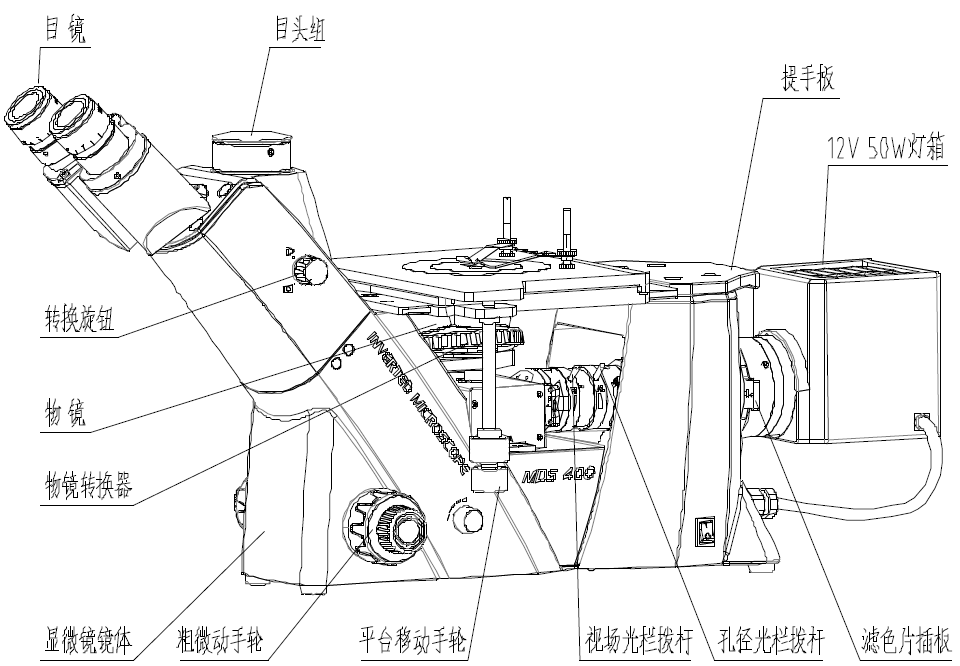
\includegraphics[width=0.9\textwidth]{MDS400.png}
        \end{figure}
\section{实验仪器}%规格及参数
    MDS400 倒置式金相显微镜,铁碳合金平衡状态金相试样一套、多种热处理方式之后的碳钢试样一套。
\section{实验过程}%简述主要过程和实验内容
    \subsection{实验内容}
        \begin{enumerate}
            \item 由指导教师结合图例讲解 Fe-C 合金平衡态的基本组织组成、组织的形态特征及金相显微镜的主要结构部件及其作用、基本操作过程及注意事项。
            \item 学生领取一套铁碳合金平衡组织标准试样,按照金相显微镜的操作步骤,在显微镜下观察表中七种铁碳合金平衡组织试样,识别碳钢和铸铁组织形态的特征,建立成分、组织之间相互关系的概念。认真体会整个操作过程,并将观察图像拍照存储。
            \item 学生领取一套经不同热处理工艺的 45 钢及 T12 钢标准试样(21\#-27\#),在显微镜下观察经不同热处理工艺的 45 钢及 T12 试样。理解并分析不同热处理工艺条件下试样的组织变化,认真体会整个操作过程,并将观察图像拍照存储。\par
            其中:\begin{enumerate}
                \item 21\# 为 45 钢 \SI{860}{\degreeCelsius} 水淬 $+$ 中温回火;
                \item 22\# 为 45 钢 \SI{860}{\degreeCelsius} 水淬 $+$ 高温回火;
                \item 23\# 为 45 钢 \SI{780}{\degreeCelsius} 水淬;
                \item 24\# 为 45 钢 \SI{1100}{\degreeCelsius} 水淬;
                \item 25\# 为 T12 钢球化退火;
                \item 26\# 为 T12 钢 \SI{780}{\degreeCelsius} 水淬 $+$ 低温回火;
                \item 27\# 为 T12 钢 \SI{1100}{\degreeCelsius} 水淬 $+$ 低温回火。
            \end{enumerate}
        \end{enumerate}
    \subsection{实验要求}
        \begin{enumerate}
            \item 通过观察金相样品的实际操作过程,学会正确的操作方法,包括物镜和目镜的选择与匹配、调焦、孔径光阑和视场光阑的调节、放大倍数的计算;
            \item 总结金相显微镜的操作要点及必须注意的事项;
            \item 给出所观察试样的显微组织图(显微镜拍摄图及手绘图),手绘图要求画出所观察显微组织示意图,显微组织画在直径为 $25$-\SI{30}{\mm} 的圆内,并标出材料、组织名称及放大倍数。
            \item  分析含碳量对铁碳合金的组织和性能的影响。
        \end{enumerate}
    \subsection{实验注意事项}
        \begin{enumerate}
            \item 操作时必须特别谨慎,不能有任何剧烈的动作,不允许自行拆卸光学系统。
            \item 在旋转粗调或微调旋钮时动作要慢,碰到某种障碍时应立即停止操作,报告指导教师查找原因,不得用力强行转动,否则会损坏机件。
            \item 要爱护已制备好的金相试样。不能用手触摸试样的观察面,如有尘埃等脏物不能用嘴吹,也不能随意擦,要用吸耳球吹除或用无水酒精冲洗并干燥。
            \item 试样观察完毕后要放入干燥箱中保存。
        \end{enumerate}
\end{document}